\section{Investigation of a Single Inverter Module}
\label{chap:curr_driven_rect}

\subsection{Power Device Stress}

As shown in Fig. \ref{fig:SingleModuleInductanceMap}, the power loop includes two switches and single phase capacitor. When the phase current transfers from one switch to the other, the power loop parasitic inductances cause a voltage overshoot on the drain-source terminals of a switch as much as $L_p*di/dt$. Due to fast switching capability (i.e. high di/dt) of GaN FETs, the power loop inductance is the most important factor for device stress. Experimental results of device stress are presented in Fig. \ref{fig:experimentalvds2} for various DC link voltages. It can be seen that the peak stress on phase-B is higher since its power loop equivalent inductance is slightly larger than phase-A.

\subsection{DC link Capacitor Stress}

The DC link capacitors on each half-bridge are used to supply and sink the current ripple during switching periods. The power loop inductances are not effective on these capacitors' stress assuming ceramic capacitors are placed in much closer proximity. When the parasitic inductances are of considerable amount on the commutation loop, the stress of individual capacitors increase due to the longer path which the other capacitors have, as shown in Fig. \ref{fig:single_module_curr_ripple}. This results in higher capacitor RMS currents than analytically calculated values in \cite{Ugur2017} as shown in Fig. \ref{fig:CapacitorCurrentRMS}. This extra ripple current can increase the capacitor temperature and shorten its lifetime. 

\begin{figure}[tb]
\minipage{0.49\textwidth}
  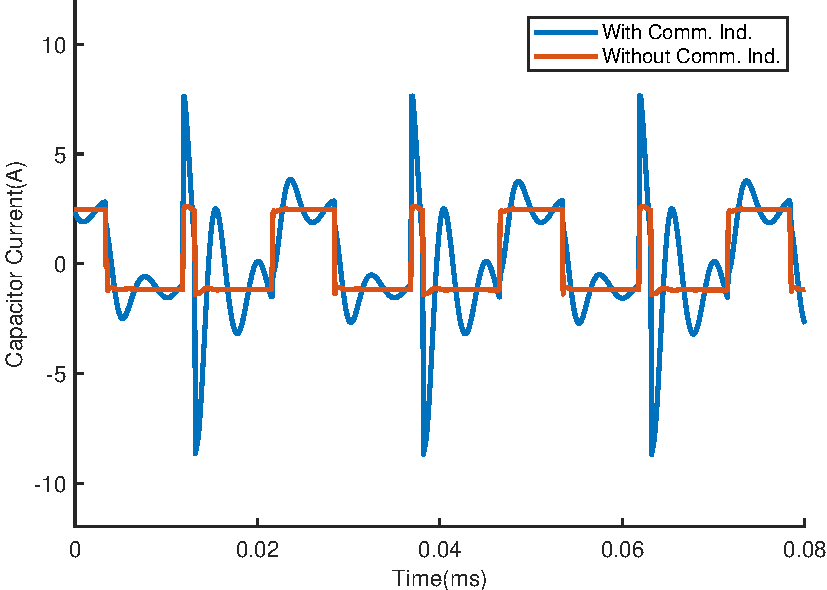
\includegraphics[width=\linewidth]{figures/single_module_curr_ripple.pdf}
  \caption{DC bus capacitor current ripple with and without commutation loop inductances}\label{fig:single_module_curr_ripple}
\endminipage\hfill
\minipage{0.49\textwidth}
  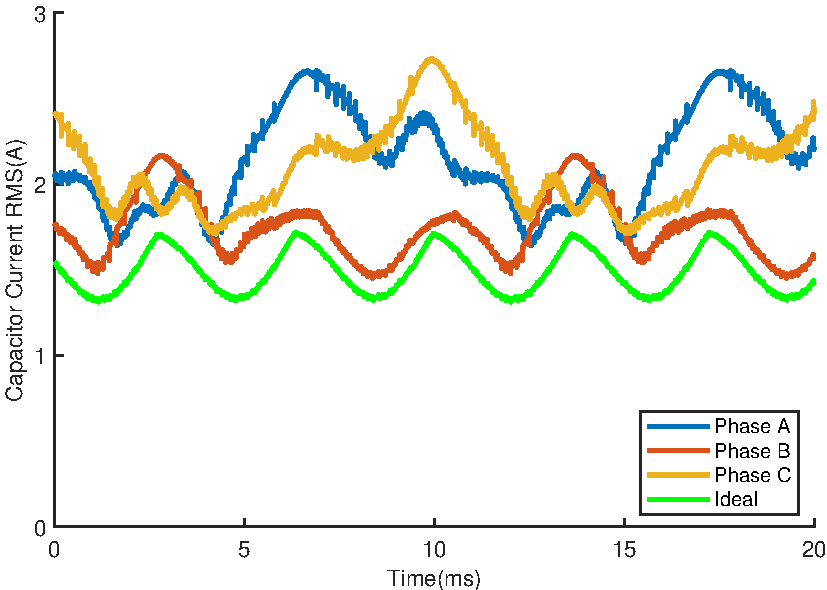
\includegraphics[width=\linewidth]{figures/CapacitorCurrentRMS.pdf}
  \caption{Variation of RMS values of capacitor currents with and without commutation inductances}\label{fig:CapacitorCurrentRMS}
\endminipage
\end{figure}


